%%%%%%%%%%%%%%%%%%%%%%%%%%%%%%%%%%%%%%%%%%%%%%%%%%%%%%%%%%%%%%%%%%%%%%%%%%%%%%%%%%%%%
% PACOTES                                                                           %
%%%%%%%%%%%%%%%%%%%%%%%%%%%%%%%%%%%%%%%%%%%%%%%%%%%%%%%%%%%%%%%%%%%%%%%%%%%%%%%%%%%%%
\documentclass[a4paper,12pt]{article}

%-----------------------------------------------------------------------------------%
% LAYOUT DA PÁGINA                                                                  %
%-----------------------------------------------------------------------------------%
\usepackage[top=3cm, bottom=3cm, left=2.5cm, right=2.5cm]{geometry}
%\usepackage{fancyhdr} % Permite controlar como são exibidos os cabeçalhos

%-----------------------------------------------------------------------------------%
% FORMATAÇÃO DO TEXTO                                                               %
%-----------------------------------------------------------------------------------%
%\usepackage{setspace} % Permite definir o espaçamento entre linhas

%-----------------------------------------------------------------------------------%
% PACOTES DE IMAGENS                                                                %
%-----------------------------------------------------------------------------------%
\usepackage[pdftex]{graphicx}
\pdfsuppresswarningpagegroup=1 % A warning issued when several PDF images are
% imported in the same page. Mostly harmless, can be almost always supressed.
%\usepackage[pstarrows]{pict2e} % Amplia as funcionalidades do ambiente picture
\usepackage{tikz}
\usetikzlibrary{shapes, arrows, arrows.meta}

%-----------------------------------------------------------------------------------%
% PACOTES DE TABELAS                                                                %
%-----------------------------------------------------------------------------------%
\usepackage{array} % Facilita a formatação de tabelas
%\usepackage{multirow} % Permite criar células que ocupam várias linhas em uma tabela
\usepackage{longtable} % Permite criar tabelas que quebram de página

%-----------------------------------------------------------------------------------%
% PACOTES MATEMÁTICOS DE BASE                                                       %
%-----------------------------------------------------------------------------------%
\usepackage{amsfonts,amstext,amscd,bezier,amsthm,amssymb}
\usepackage[centertags]{amsmath}

%-----------------------------------------------------------------------------------%
% PACOTES DE SÍMBOLOS MATEMÁTICOS                                                   %
%-----------------------------------------------------------------------------------%
%\usepackage{mathtools} % Símbolos matemáticos extras. (ex.: \xrightharpoon)
%\usepackage[integrals]{wasysym} % Muda o estilo das integrais, além de outros
%                                 símbolos extras
%\usepackage[nice]{nicefrac} % Permite o uso de frações "melhores". Usar \nicefrac{}{}

%-----------------------------------------------------------------------------------%
% PACOTES DE FONTES MATEMÁTICAS                                                     %
%-----------------------------------------------------------------------------------%
%\usepackage{mathbbol} % Quase todos os símbolos com \mathbb
%\usepackage{bbm} % Extensão dos símbolos de \mathbb. Usar comando \mathbbm
%\usepackage{calrsfs} % Muda o estilo de \mathcal
%\usepackage[mathcal]{euscript} % Muda o estilo de \mathcal

%-----------------------------------------------------------------------------------%
% PACOTES DE CODIFICAÇÃO DE FONTES                                                  %
%-----------------------------------------------------------------------------------%
\usepackage[utf8]{inputenc} % Permite o uso de caracteres ISO 8859-1, incluindo os
%                               caracteres acentuados diretamente.
\usepackage[T1]{fontenc} % Uso de fontes T1, necessário para tratar caracteres
%                          acentuados como um único bloco.

%-----------------------------------------------------------------------------------%
% PACOTES DE LÍNGUAS                                                                %
%-----------------------------------------------------------------------------------%
\usepackage[french]{babel} % Seleciona a língua do documento, definindo nomes de
%                              seções, nome do índice, da bibliografia, etc. Em caso
%                              de documento com mais de uma língua, a padrão é a
%                              última.
\NoAutoSpaceBeforeFDP % Utilizar em francês se quiser evitar espaços antes de :

%-----------------------------------------------------------------------------------%
% PACOTES DE BIBLIOGRAFIA                                                           %
%-----------------------------------------------------------------------------------%
%\usepackage{babelbib} % Permite definir a língua das entradas da bibliografia. Usar
%                       [fixlanguage] para uma mesma língua para todas as entradas e
%                       \selectbiblanguage{} para definir a língua. Um estilo compa-
%                       tível com babelbib deve ser usado (ex: babplain)
\usepackage{cite} % Organiza os elementos citados dentro de um mesmo \cite.

%-----------------------------------------------------------------------------------%
% PACOTES DE FONTES                                                                 %
%-----------------------------------------------------------------------------------%
% Computer Modern (fonte padrão)                                                    %
% - - - - - - - - - - - - - - - - - - - - - - - - - - - - - - - - - - - - - - - - - %
%\usepackage{ae} % A usar com a fonte padrão do LaTeX quando forem gerados PDFs, para
%                 corrigir erros de visualização

% Computer Modern Bright (sans serif)                                               %
% - - - - - - - - - - - - - - - - - - - - - - - - - - - - - - - - - - - - - - - - - %
%\usepackage{cmbright}

% Times New Roman                                                                   %
% - - - - - - - - - - - - - - - - - - - - - - - - - - - - - - - - - - - - - - - - - %
%\usepackage{mathptmx} % Muda texto e modo matemático
%\usepackage{times} % Apenas texto, não muda modo matemático

% Arial                                                                             %
% - - - - - - - - - - - - - - - - - - - - - - - - - - - - - - - - - - - - - - - - - %
%\usepackage[scaled]{uarial} % Arial como fonte sans serif padrão

% Palatino                                                                          %
% - - - - - - - - - - - - - - - - - - - - - - - - - - - - - - - - - - - - - - - - - %
%\usepackage{mathpazo} % Muda texto e modo matemático
%\usepackage{palatino} % Apenas texto, não muda modo matemático

% Concrete                                                                          %
% - - - - - - - - - - - - - - - - - - - - - - - - - - - - - - - - - - - - - - - - - %
%\usepackage{ccfonts} % Texto: Concrete; Matemático: Concrete Math
%\usepackage{ccfonts, eulervm} % Texto: Concrete; Matemático: Euler

% Iwona                                                                             %
% - - - - - - - - - - - - - - - - - - - - - - - - - - - - - - - - - - - - - - - - - %
%\usepackage[math]{iwona} % Texto e modo matemático: Iwona

% Kurier                                                                            %
% - - - - - - - - - - - - - - - - - - - - - - - - - - - - - - - - - - - - - - - - - %
%\usepackage[math]{kurier} % Texto e modo matemático: Kurier

% Antykwa Póltawskiego                                                              %
% - - - - - - - - - - - - - - - - - - - - - - - - - - - - - - - - - - - - - - - - - %
%\usepackage{antpolt} % Texto: Antykwa Póltawskiego; Matemático: nenhum
                     % Usar fontenc = QX ou OT4

% Utopia                                                                            %
% - - - - - - - - - - - - - - - - - - - - - - - - - - - - - - - - - - - - - - - - - %                     
%\usepackage{fourier} % Texto: Utopia; Matemático: Fourier

% KP Serif                                                                          %
% - - - - - - - - - - - - - - - - - - - - - - - - - - - - - - - - - - - - - - - - - %
\usepackage{kpfonts}

%-----------------------------------------------------------------------------------%
% CORES                                                                             %
%-----------------------------------------------------------------------------------%
\usepackage{color}
\definecolor{darkgreen}{rgb}{0,0.5,0}
\definecolor{darkmagenta}{rgb}{0.5,0,0.5}
\definecolor{darkgray}{rgb}{0.5,0.5,0.5}
\definecolor{darkblue}{rgb}{0.2,0.2,0.4}
\definecolor{darkred}{rgb}{0.6,0.15,0.15}
\definecolor{gray}{rgb}{0.65,0.65,0.65}
\definecolor{lightgray}{rgb}{0.8,0.8,0.8}
\definecolor{lightblue}{rgb}{0.5,0.5,1}
\definecolor{lightgreen}{rgb}{0.5,1,0.5}
\definecolor{deadred}{rgb}{0.7, 0.2, 0.2}
\definecolor{deadblue}{rgb}{0.2, 0.2, 0.7}

%-----------------------------------------------------------------------------------%
% PACOTES DIVERSOS                                                                  %
%-----------------------------------------------------------------------------------%
\usepackage{icomma} % Permite uso de vírgula como separador decimal
\usepackage{url} % Pacote para não ter problemas com URLs. Usar \url{}
%\usepackage{randtext} % Troca a ordem de letras de uma frase (útil com e-mails em
                      % PDFs a serem publicados on-line.
\usepackage[hidelinks]{hyperref}
%\usepackage{showkeys} % Para mostrar o nome dos labels
\usepackage{enumitem} % Facilita o uso de listas, inclusive referências a itens de
                      % listas.
%\usepackage[absolute]{textpos} % Posição absoluta de texto na página
%\usepackage{pdfpages} % Permite incluir documentos em PDF no arquivo
%\usepackage{refcheck} % Verifica as referências procurando por
%                      % labels não usados ou equações numeradas sem labels.
%                      % Verificar o arquivo .log e procurar por RefCheck.
%\usepackage[french]{algorithm2e}

%%%%%%%%%%%%%%%%%%%%%%%%%%%%%%%%%%%%%%%%%%%%%%%%%%%%%%%%%%%%%%%%%%%%%%%%%%%%%%%%%%%%%
% CONFIGURAÇÕES                                                                     %
%%%%%%%%%%%%%%%%%%%%%%%%%%%%%%%%%%%%%%%%%%%%%%%%%%%%%%%%%%%%%%%%%%%%%%%%%%%%%%%%%%%%%

%-----------------------------------------------------------------------------------%
% FORMATAÇÃO DO TEXTO                                                               %
%-----------------------------------------------------------------------------------%
%\onehalfspacing % Espaçamento 1 1/2 (definido no pacote setspace)

%-----------------------------------------------------------------------------------%
% DEFINIÇÃO DE AMBIENTES MATEMÁTICOS                                                %
%-----------------------------------------------------------------------------------%
%\theoremstyle{plain}
%\newtheorem{theo}{Teorema}[section]
%\newtheorem{lemm}[theo]{Lema}
%\newtheorem{coro}[theo]{Corolário}
%\newtheorem{prop}[theo]{Proposição}
%\theoremstyle{definition}
%\newtheorem{defi}[theo]{Definição}
%\newtheorem{remq}[theo]{Observação}
%%\newtheorem{expl}[theo]{Exemplo}
%\newenvironment{expl}%
%  {\refstepcounter{theo}%
%    \begin{list}{}{%
%    \setlength{\topsep}{0pt}%
%    \setlength{\leftmargin}{\parindent}%
%    \setlength{\rightmargin}{0pt}%
%    \setlength{\listparindent}{\parindent}%
%    \setlength{\itemindent}{0pt}%
%    \setlength{\parsep}{\parskip}}%
%    \item[]{\bf Exemplo \thetheo. }}%
%  {\hspace*{\fill} $\square$ \end{list} \medskip}
%\newenvironment{solu}%
%  {\noindent {\bf Solução. }\small}%
%  {\hspace*{\fill} $\square$ \normalsize \medskip}
%\newenvironment{dems}[1][Demonstração]%
%  {\begin{list}{}{%
%    \setlength{\topsep}{0pt}%
%    \setlength{\leftmargin}{\parindent}%
%    \setlength{\rightmargin}{0pt}%
%    \setlength{\listparindent}{\parindent}%
%    \setlength{\itemindent}{0pt}%
%    \setlength{\parsep}{\parskip}}%
%    \item[]{\bf #1. }}%
%  {\hspace*{\fill} $\blacksquare$ \end{list} \medskip}


%-----------------------------------------------------------------------------------%
% DEFINIÇÃO DE COMANDOS MATEMÁTICOS                                                 %
%-----------------------------------------------------------------------------------%
%\newcommand*\diff{\mathop{}\!\mathrm{d}}

%\newcommand{\norm}[1]{\left\lVert #1\right\lVert} % Norma
%\newcommand{\abs}[1]{\left\lvert #1\right \rvert} % Valor absoluto
%\newcommand{\floor}[1]{\left\lfloor #1 \right\rfloor} % Arredondar para baixo
%\newcommand{\ceil}[1]{\left\lceil #1 \right\rceil} % Arredondar para cima


%-----------------------------------------------------------------------------------%
% NUMERAÇÃO DE ELEMENTOS                                                            %
%-----------------------------------------------------------------------------------%
%\numberwithin{table}{section}
%\numberwithin{table}{subsection}
%\numberwithin{figure}{section}
%\numberwithin{figure}{subsection}
\numberwithin{equation}{section}
%\numberwithin{equation}{subsection}
%\numberwithin{theo}{chapter}
%\numberwithin{theo}{subsection}

%%%%%%%%%%%%%%%%%%%%%%%%%%%%%%%%%%%%%%%%%%%%%%%%%%%%%%%%%%%%%%%%%%%%%%%%%%%%%%%%%%%%%
% ESTRUTURA DO DOCUMENTO                                                            %
%%%%%%%%%%%%%%%%%%%%%%%%%%%%%%%%%%%%%%%%%%%%%%%%%%%%%%%%%%%%%%%%%%%%%%%%%%%%%%%%%%%%%
\begin{document}

\title{2I006 \\ Projet : Le Robot Trieur}
\author{Ariana Carnielli et Lisa Kacel}
\date{}

\maketitle

\section{Introduction}

Ce projet s'intéresse à la recherche automatique des solutions pour le jeu du ``robot trieur''. Dans ce jeu, un robot se déplace dans un grille à $m$ lignes et $n$ colonnes. Chaque case possède une couleur de fond et peut comporter une pièce colorée, le nombre de cases et pièces d'une même couleur étant identique. Le robot peut porter au plus une pièce, il peut se déplacer d'une case à toutes les cases voisines, et peut échanger la pièce qu'il porte contre la pièce dans la case où il est, prendre la pièce de la case où il est s'il ne porte pas déjà une pièce, ou laisser la pièce qu'il porte dans la case où il est si celle-ci n'a pas déjà une pièce. L'objectif du jeu est de ranger chaque pièce dans une case de même couleur. Une case comportant une pièce de même couleur que son fond est appelée \emph{noire}. L'implémentation du jeu a été fournie pour ce projet.

\section{Première partie : Algorithme ``au plus proche''}
\label{SecAuPlusProche}

L'objectif de cette première partie du projet est de donner quelques implémentations différentes d'un algorithme pour résoudre le problème, appelé algorithme ``au plus proche'', et comparer leurs complexités et vitesses d'exécution.

L'algorithme ``au plus proche'' consiste à, tant qu'il reste une case non-noire, vérifier si le robot porte une pièce ou pas. S'il porte une pièce, le robot se déplace à la case la plus proche avec la même couleur de fond que la pièce et la dépose. Sinon, il cherche la plus proche case non-noire avec une pièce et se déplace pour la prendre. En cas d'égalité de distance, la priorité est donnée à la case en haut, à gauche. Les implémentations diffèrent par la méthode utilisée pour trouver la case la plus proche où se déplacer.

Il est intéressant à noter que cet algorithme ne donne pas forcément la solution avec le nombre minimal de déplacements. En effet, considérons l'exemple de la grille de la Figure \ref{FigExpl}. On note les déplacements du robot vers le haut, le bas, la gauche et la droite respectivement par \texttt{U}, \texttt{D}, \texttt{L} et \texttt{R}, et l'échange de pièce du robot par \texttt{S}. Si le robot se trouve initialement à la case en haut à gauche, une application de l'algorithme ``au plus proche'' donne la solution suivante, à 10 déplacements :

\texttt{S R S L S R R S R S D S L S L S U R S}

Néanmoins, une autre solution possible, à 7 déplacements, est :

\texttt{S R R S R S D S L S L S U S}

On remarque par cet exemple que chercher à chaque fois la case la plus proche avec la même couleur peut ne pas donner la solution optimale.

\begin{figure}[ht]
\centering
\begin{tikzpicture}
\fill[black] (0, 0) -- (2, 0) -- (2, 2) -- (0, 2);
\fill[violet] (2, 0) -- (4, 0) -- (4, 2) -- (2, 2);
\fill[red!50!yellow] (4, 0) -- (6, 0) -- (6, 2) -- (4, 2);
\fill[green] (6, 0) -- (8, 0) -- (8, 2) -- (6, 2);
\fill[blue] (0, 2) -- (2, 2) -- (2, 4) -- (0, 4);
\fill[yellow] (2, 2) -- (4, 2) -- (4, 4) -- (2, 4);
\fill[yellow] (4, 2) -- (6, 2) -- (6, 4) -- (4, 4);
\fill[red] (6, 2) -- (8, 2) -- (8, 4) -- (6, 4);

\fill[yellow] (2.5, 0.5) -- (3.5, 0.5) -- (3.5, 1.5) -- (2.5, 1.5);
\fill[violet] (4.5, 0.5) -- (5.5, 0.5) -- (5.5, 1.5) -- (4.5, 1.5);
\fill[red!50!yellow] (6.5, 0.5) -- (7.5, 0.5) -- (7.5, 1.5) -- (6.5, 1.5);
\fill[yellow] (0.5, 2.5) -- (1.5, 2.5) -- (1.5, 3.5) -- (0.5, 3.5);
\fill[blue] (2.5, 2.5) -- (3.5, 2.5) -- (3.5, 3.5) -- (2.5, 3.5);
\fill[red] (4.5, 2.5) -- (5.5, 2.5) -- (5.5, 3.5) -- (4.5, 3.5);
\fill[green] (6.5, 2.5) -- (7.5, 2.5) -- (7.5, 3.5) -- (6.5, 3.5);
\end{tikzpicture}
\caption{Exemple de grille où l'algorithme ``au plus proche'' ne donne pas le nombre minimal de déplacements.}
\label{FigExpl}
\end{figure}

\subsection{Version naïve}
\label{SecNaive}

La première méthode utilisée pour chercher la case la plus proche est celle dite \emph{naïve}, qui consiste à parcourir, à chaque fois, toute la grille du jeu à partir de la case $(0, 0)$ afin de trouver la case la plus proche à la case où le robot se trouve. On a pour cela implémenté plusieurs fonctions utiles dans une bibliothèque de fonctions : la fonction \verb@PlusCourtChemin@ de la Question 1.2 et des petites fonctions qui aident à rendre le code plus lisible. La plupart d'entre elles retourne des booléens utilisés pour décider où le robot va se déplacer. En particulier, on a implémenté des fonctions répondant à la Question 1.3.

On a implémenté deux fonctions \verb@RechercheCaseNaif_c@ et \verb@RechercheCaseNaif_nn@ qui retournent les coordonnées $(k, l)$, respectivement, de la case la plus proche d'une case $(i, j)$ donnée et dont la couleur de fond est une couleur $c$ donnée, et de la case la plus proche de $(i, j)$ non-noire et comportant une pièce. On a utilisé ces deux fonctions et les fonctions données pour implémenter une résolution par l'algorithme ``au plus proche''. On a aussi crée un programme principal \verb@Solveur@ qui prend en argument les dimensions de la grille, le nombre de couleurs, la graine pour le générateur aléatoire et le numéro du solveur à utiliser (1 pour le solveur naïf, d'autres numéros ayant été ajoutés pour les solveurs implémentés dans les sections suivantes) et qui enregistre la solution trouvée dans un fichier.

Pour toutes les simulations de temps d'exécution de ce rapport, nous avons désactivé l'enregistrement de la solution (après avoir vérifié que la solution enregistrée était bonne) afin de mesurer uniquement le temps de calcul et ne pas avoir des structures de solution occupant trop de mémoire pour les dimensions importantes de grille. Le nombre de couleurs a été choisi comme étant égal à $10$ pour toutes les simulations, et le temps d'exécution donné dans les Tables \ref{TempsNaive} à \ref{TempsAVL} correspond à une moyenne sur 4 simulations pour chaque dimension de la grille.

Expérimentalement, en utilisant la fonction \verb@clock@ de la bibliothèque \verb@time.h@, on a trouvé les temps d'exécution de la Table \ref{TempsNaive}. On remarque que le temps moyen d'exécution dépasse les $30 s$ pour des grilles de taille d'environ $270 \times 270$.

\begin{table}[ht]
\centering
\begin{tabular}{cc}
\hline\hline
Dimensions de la grille & Temps moyen d'exécution \tabularnewline
\hline
$250 \times 250$ & $22,62 s$ \tabularnewline
$260 \times 260$ & $26,89 s$ \tabularnewline
$270 \times 270$ & $30,37 s$ \tabularnewline
\hline\hline
\end{tabular}
\caption{Temps d'exécution de la version naïve.}
\label{TempsNaive}
\end{table}

\subsection{Version circulaire}

La méthode circulaire de recherche de la case $(k, l)$ la plus proche d'une case $(i, j)$ donnée consiste à démarrer la recherche depuis $(i, j)$ et chercher de façon circulaire, en augmentant la distance de $1$ à chaque fois jusqu'à ce qu'une case avec la propriété voulue soit trouvée. Par rapport à la version naïve, l'avantage est que l'on peut arrêter la recherche dès qu'une première case est trouvée, sans avoir besoin de parcourir toute la grille.

On a implémenté les deux fonctions \verb@RechercheCaseCirculaire_c@ et \verb@Recherche@\allowbreak\verb@CaseCirculaire_nn@, analogues à celles implémentées pour la version naïve, et un solveur les utilisant. Les résultats expérimentaux de temps moyens d'exécution sur 4 simulations sont données dans la Table \ref{TempsCirculaire}, qui les compare avec les résultats de la Table \ref{TempsNaive}. On remarque que le temps d'exécution moyen de la version circulaire est plus petit, car la recherche s'arrête dès qu'une case a été trouvée. On peut donc résoudre des grilles de dimension jusqu'à environ $330 \times 330$ en moins de $30 s$.

\begin{table}[ht]
\centering
\begin{tabular}{>{\centering} m{0.3\textwidth} >{\centering} m{0.3\textwidth} >{\centering} m{0.3\textwidth}}
\hline\hline
Dimensions de la grille & Temps moyen d'exécution, version naïve & Temps moyen d'exécution, version circulaire \tabularnewline
\hline
$250 \times 250$ & $22,62 s$ & $10,02 s$ \tabularnewline
$260 \times 260$ & $26,89 s$ & $10,64 s$ \tabularnewline
$270 \times 270$ & $30,37 s$ & $12,73 s$ \tabularnewline
$320 \times 320$ &           & $26,88 s$ \tabularnewline
$330 \times 330$ &           & $30,94 s$ \tabularnewline
$340 \times 340$ &           & $34,98 s$ \tabularnewline
\hline\hline
\end{tabular}
\caption{Temps d'exécution des versions naïve et circulaire.}
\label{TempsCirculaire}
\end{table}

On a aussi fait des tests en augmentant le nombre de couleurs pour une taille fixé de la grille. On observe que, comme attendu, le temps d'exécution de la méthode naïve reste constant, car il parcourt toujours toutes les cases de la grille pour une recherche. Néanmoins, le temps d'exécution de la méthode circulaire augmente, car, avec plus de couleurs, il lui faut en moyenne chercher plus loin pour trouver une case.

Pour la complexité de la méthode naïve dans le cas d'une grille $n \times n$, la recherche parcourt toujours toutes les $n^2$ cases de la grille, et est ainsi effectuée en $\Theta(n^2)$. Pour résoudre la grille, il faut effectuer cette recherche une fois pour chaque pièce de la grille, soit $n^2$ pièces, donc la complexité est en $\Theta(n^4)$.

Pour la méthode circulaire, le pire cas correspond à lorsque la case recherchée est le plus éloignée possible de la case courante, auquel cas il faut parcourir toutes les $n^2$ cases de la grille, mais elle peut être plus courte, lorsque par exemple la case recherchée est voisine de la case courante. On a donc une complexité de $O(n^2)$. Comme pour la méthode naïve, il faut effectuer la recherche une fois pour chacune des $n^2$ pièces, donnant donc une complexité en $O(n^4)$.

Les expérimentations permettent de retrouver cette évaluation de la complexité. Pour la méthode naïve, en utilisant la première et la troisième lignes du tableau, on obtient $\frac{31,36 s}{22,94 s} \approx 1,34$ et $\left(\frac{270}{250}\right)^4 \approx 1,36$, ce qui valide la complexité en $\Theta(n^4)$. De même, pour la méthode circulaire, en utilisant la première et la dernière lignes du tableau, on obtient $\frac{34,98 s}{10,02 s} \approx 3,49$ et $\left(\frac{340}{250}\right)^4 \approx 3,42$, ce qui valide également le calcul théorique de la complexité en $O(n^4)$.

\subsection{Version par couleur}
\label{SecCouleur}

La méthode par couleur consiste à créer un tableau de dimension 1 et longueur égale à la quantité de couleurs et contenant dans chaque case une liste doublement chainée avec les indices des cases ayant une même couleur de fond. Pour effectuer la recherche de la case la plus proche d'une couleur donnée, il suffit de parcourir la liste chainée correspondante. On ne fait donc un parcours complet de la grille qu'une seule fois, pour la construction du tableau de listes. Néanmoins, on utilise encore la méthode circulaire pour trouver une case non-noire contenant une pièce.

On a commencé par implémenter une bibliothèque de fonctions pour la manipulation de listes chainées, avec des fonctions d'initialisation, insertion en queue en $\Theta(1)$, suppression en $\Theta(1)$, affichage, etc. Ensuite, on a implémenté la fonction \verb@LDC@\allowbreak\verb@rechercherPlusProcheCase@ de recherche de case plus proche d'une case $(i, j)$ passée en argument. Cette fonction parcourt toute la liste chainée passée en argument pour trouver la case la plus proche.

En utilisant cette fonction et la fonction \verb@Recherche@\allowbreak\verb@CaseCirculaire_nn@ de la partie précédente, on a implémenté un nouveau solveur pour résoudre le robot trieur. Les résultats expérimentaux des temps moyen d'exécution sont donnés dans la Table \ref{TempsCouleur}. On remarque que le temps d'exécution moyen est beaucoup plus petit que pour les deux autres versions, étant de l'ordre de $30 s$ pour des grilles de taille d'environ $590 \times 590$.

\begin{table}[ht]
\centering
\begin{tabular}{>{\centering} m{0.2\textwidth} >{\centering} m{0.2\textwidth} >{\centering} m{0.2\textwidth} >{\centering} m{0.2\textwidth}}
\hline\hline
Dimensions de la grille & Temps moyen, version naïve & Temps moyen, version circulaire & Temps moyen, version par couleur \tabularnewline
\hline
$250 \times 250$ & $22,62 s$ & $10,02 s$ & $1,055 s$ \tabularnewline
$260 \times 260$ & $26,89 s$ & $10,64 s$ & $1,176 s$ \tabularnewline
$270 \times 270$ & $30,37 s$ & $12,73 s$ & $1,441 s$ \tabularnewline
$320 \times 320$ &           & $26,88 s$ & $2,984 s$ \tabularnewline
$330 \times 330$ &           & $30,94 s$ & $3,113 s$ \tabularnewline
$340 \times 340$ &           & $34,98 s$ & $3,313 s$ \tabularnewline
$580 \times 580$ &           &           & $28,71 s$ \tabularnewline
$590 \times 590$ &           &           & $30,48 s$ \tabularnewline
$600 \times 600$ &           &           & $33,04 s$ \tabularnewline
\hline\hline
\end{tabular}
\caption{Temps d'exécution des versions naïve, circulaire et par couleur.}
\label{TempsCouleur}
\end{table}

Étudions la complexité de la méthode par couleur en fonction de $n$ et du nombre maximal de pièces d'une même couleur $\alpha$. Pour initialiser le tableau de listes chainées, il faut parcourir la grille une fois, la complexité de cette étape étant donc en $\Theta(n^2)$. Pour rechercher la case la plus proche de couleur $c$, il faut parcourir une fois la liste chainée de la couleur correspondante, et alors la complexité est $\Theta(\ell_c)$, où $\ell_c$ est la longueur de cette liste. Comme $\alpha$ est la taille de la plus grande liste, on obtient ainsi une complexité en $O(\alpha)$ pour la recherche. Comme il faut répéter la recherche pour les $n^2$ pièces, en prenant en compte aussi l'initialisation, la complexité totale est en $\Theta(n^2) + O(n^2 \alpha) = O(n^2 \alpha)$. La taille $\alpha$ de la plus grande liste est bornée par le nombre de pièces $n^2$ et ainsi, en fonction de $n$, on a une complexité en $O(n^4)$.

\subsection{Version par AVL}
\label{SecAVL}

Dans la méthode par AVL, on utilise des arbres binaires de recherche équilibrées du type AVL pour faciliter la recherche de la case la plus proche avec une couleur donnée. Plus précisément, on crée un tableau \verb@M@ d'arbres AVL de dimension \verb@m@ $\times$ \verb@nb_coul@, où \verb@m@ est le nombre de lignes de la grille et \verb@nb_coul@ le nombre de couleurs utilisées dans la grille. L'arbre \verb@M[i][c]@ contient les indices de colonne \verb@j@ de toutes les cases de la grille dans la ligne \verb@i@ et de couleur de fond \verb@c@.

On a commencé par l'implémentation d'une bibliothèque pour la manipulation d'arbres AVL, avec des fonctions d'initialisation, insertion en $O(\log(\beta))$ (où $\beta$ est la quantité d'éléments de l'arbre), suppression en $O(\log(\beta))$, rotations droite et gauche en $O(1)$, équilibrage d'un n\oe{}ud en $O(1)$, affichage, etc. Les fonctions de cette bibliothèque ont été testées en insérant, recherchant et supprimant plusieurs éléments d'un arbre.

On a également implémenté une fonction de recherche qui, étant donné un arbre AVL à entrées positives ou nulles et un entier $c$, recherche et retourne l'entier le plus proche de $c$ dans l'arbre (ou $-1$ si l'arbre est vide). Dans le cas où deux entiers de l'arbre sont à même distance de $c$, on retourne le plus petit. Cette fonction utilise une recherche dichotomique : si la valeur $c$ est plus petite que la racine de l'arbre, alors l'élément de l'arbre le plus proche de $c$ est soit sa racine, soit un élément de son sous-arbre gauche, avec la situation symétrique lorsque $c$ est plus grand que la racine de l'arbre. Une implémentation récursive de cette fonction de recherche permet ainsi d'avoir une complexité en $O(h)$, où $h$ est la hauteur de l'arbre, et donc en $O(\log(\beta))$ puisqu'un arbre AVL est équilibré.

Pour utiliser cette structure dans l'implémentation de l'algorithme ``au plus proche'', on a écrit une fonction de création du tableau d'arbres AVL \verb@M@ à partir d'une grille. Cette fonction parcourt toute la grille en insérant, pour les cases non-noires, son indice de colonne dans l'arbre correspondant à sa couleur de fond. On a aussi décidé de rajouter une dernière colonne à \verb@M@ contenant, pour chaque ligne, un arbre avec les indices de toutes les cases non-noires avec une pièce de la ligne, afin de pouvoir implémenter efficacement la recherche de cases non-noires.

On a en plus implémenté des fonctions de recherche de case par couleur et de recherche de cases non-noires avec une pièce afin d'implémenter l'algorithme ``au plus proche'' par AVL. Pour les recherches de la case la plus proche, on parcourt les lignes du tableau \verb@M@ et, pour chaque ligne, on recherche la colonne la plus proche dans l'arbre AVL de la couleur correspondante, gardant à la fin la distance minimale par rapport à toutes les lignes. Le test du temps moyen d'exécution est donné dans la Table \ref{TempsAVL}.

\begin{table}
\centering
\begin{tabular}{>{\centering} m{0.17\textwidth} >{\centering} m{0.17\textwidth} >{\centering} m{0.17\textwidth} >{\centering} m{0.17\textwidth} >{\centering} m{0.17\textwidth}}
\hline\hline
Dimensions de la grille & Version naïve & Version circulaire & Version par couleur & Version par AVL \tabularnewline
\hline
$250 \times 250$   & $22,62 s$ & $10,02 s$ & $1,055 s$ & $0,3672 s$ \tabularnewline
$260 \times 260$   & $26,89 s$ & $10,64 s$ & $1,176 s$ & $0,4063 s$ \tabularnewline
$270 \times 270$   & $30,37 s$ & $12,73 s$ & $1,441 s$ & $0,4961 s$ \tabularnewline
$320 \times 320$   &           & $26,88 s$ & $2,984 s$ & $0,7617 s$ \tabularnewline
$330 \times 330$   &           & $30,94 s$ & $3,113 s$ & $0,8203 s$ \tabularnewline
$340 \times 340$   &           & $34,98 s$ & $3,313 s$ & $0,9023 s$ \tabularnewline
$580 \times 580$   &           &           & $28,71 s$ & $4,629 s$  \tabularnewline
$590 \times 590$   &           &           & $30,48 s$ & $4,965 s$  \tabularnewline
$600 \times 600$   &           &           & $33,04 s$ & $5,281 s$  \tabularnewline
$1000 \times 1000$ &           &           &           & $26,95 s$  \tabularnewline
$1050 \times 1050$ &           &           &           & $32,41 s$  \tabularnewline
$1100 \times 1100$ &           &           &           & $38,50 s$  \tabularnewline
\hline\hline
\end{tabular}
\caption{Temps d'exécution des versions naïve, circulaire, par couleur et par AVL.}
\label{TempsAVL}
\end{table}

En comparant avec la méthode par couleur, on remarque que la méthode par AVL est plus rapide. La dimension de la grille qui donne un temps moyen d'exécution de $30 s$ est entre $1000 \times 1000$ et $1050 \times 1050$.

La complexité de la création du tableau d'AVL est en $O(n^2 \log(\beta))$, où $\beta$ est le nom\-bre maximal d'éléments dans un arbre AVL du tableau. Il faut parcourir les $n^2$ éléments de la grille et les insérer dans un AVL, l'insertion étant faite, comme vu précédemment, en $O(\log(\beta))$. La complexité de la recherche de la case la plus proche par AVL est en $O(n \log(\beta))$. En effet, on fait une boucle sur les $n$ lignes du tableau \verb@M@ et, pour chaque ligne, on fait une recherche uniquement sur l'arbre de la couleur correspondante, qui se fait en $O(\log(\beta))$. Comme cette recherche est répétée pour les $n^2$ pièces de la grille, on a une complexité totale en $O(n^2 \log(\beta)) + O(n^3 \log(\beta)) = O(n^3 \log(\beta))$. Le nombre d'éléments $\beta$ du plus grand AVL est borné par le nombre de pièces $n$ d'une ligne et ainsi, en fonction de $n$, on a une complexité en $O(n^3 \log(n))$.

La Figure \ref{FigGraphes} donne les graphes des temps d'exécution de l'algorithme ``au plus proche'' pour les quatre méthodes précédentes. Pour chaque dimension $n \times n$ de la grille, les simulations ont été répétées 10 fois, le temps donné dans le graphique étant le temps moyen d'exécution. Comme montré par les calculs théoriques de complexité des questions précédentes, la méthode naïve est en $\Theta(n^4)$, les méthodes circulaire et par couleur sont en $O(n^4)$, et la méthode par AVL est plus rapide, en $O(n^3 \log(n))$. Parmi les méthodes qui ont la même complexité en $n^4$, les améliorations des méthodes circulaire et par couleur permettent de réduire le temps d'exécution par rapport à la méthode naïve.

\begin{figure}[ht]
\centering
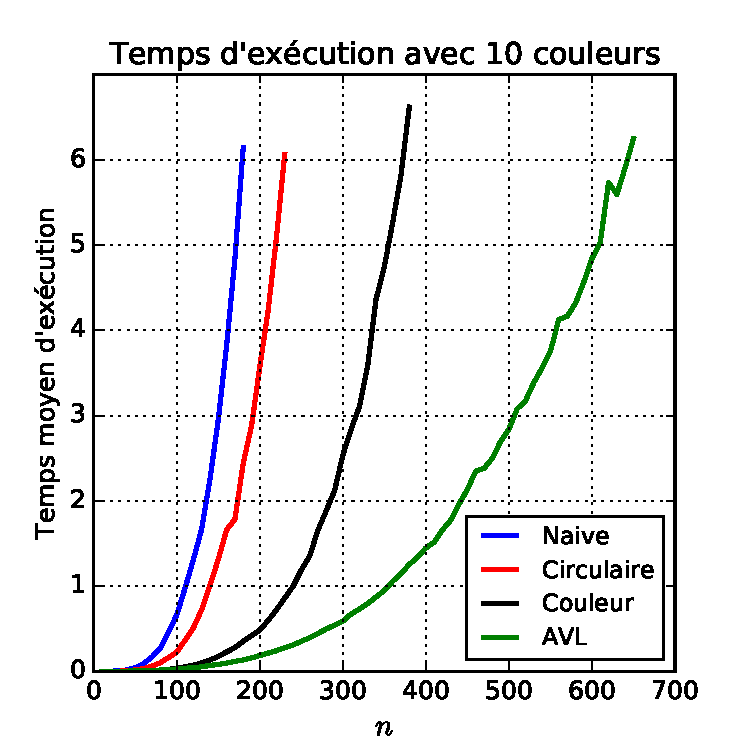
\includegraphics[width=0.7\textwidth]{Temps.pdf}
\caption{Temps d'exécution des quatre méthodes différentes.}
\label{FigGraphes}
\end{figure}

\section{Deuxième partie : Grilles de jeu à une case par couleur}

Dans cette deuxième partie, on s'est intéressé au cas particulier où la grille satisfait deux conditions : d'une part, elle n'est composée que d'une seule ligne, c'est-à-dire $m = 1$, et, d'autre part, il n'y a qu'une seule pièce et une seule case par couleur, c'est-à-dire $n = {}$\verb@nb_coul@. Ce choix simplificateur est motivé par l'existence d'un algorithme polynomial pour résoudre une telle grille avec le nombre minimal de déplacements.

L'implémentation de cet algorithme nécessite une décomposition en circuits d'un graphe sous-jacent à la grille. La construction de ce graphe et la décomposition en circuits sont indépendantes des conditions supplémentaires sur la grille, et ont donc été implémentées en toute généralité. La description de cette implémentation est donnée dans la Section \ref{SecGrapheCircuits}. L'implémentation de l'algorithme en soi est décrite dans la Section \ref{SecAlgo}.

\subsection{Graphe et circuit}
\label{SecGrapheCircuits}

\subsubsection*{Graphe}

Un graphe $H = (V, A)$ est obtenu à partir d'une grille $G$ de la façon suivante : chaque case de la grille est un sommet de $H$ et il y a un arc du sommet $(i, j)$ au sommet $(i^\prime, j^\prime)$ si et seulement si ces deux sommets correspondent à des cases non-noires et la pièce dans $(i, j)$ a la même couleur que le fond de $(i^\prime, j^\prime)$. Ainsi, la grille de la Figure \ref{FigGrilleGraphe}(a), obtenue avec $m = 3$, $n = 3$, \verb@nb_coul@${} = 4$ et la graine aléatoire $0$, donne le graphe de la Figure \ref{FigGrilleGraphe}(b).

\begin{figure}
\centering
\begin{tabular}{@{} >{\centering} m{0.5\textwidth} @{} >{\centering} m{0.5\textwidth} @{}}
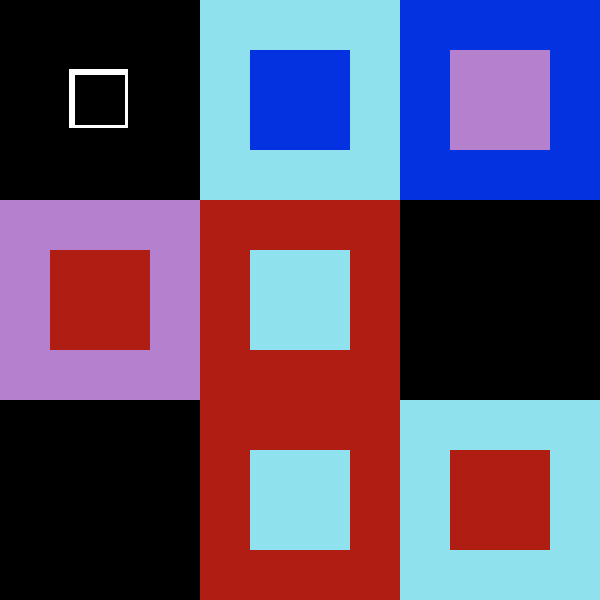
\includegraphics[width=0.4\textwidth]{3_3_4_0} & \begin{tikzpicture}
\node[circle, draw, thick] (A) at (2, 0) {};
\node[circle, draw, thick] (B) at (4, 0) {};
\node[circle, draw, thick] (C) at (0, 2) {};
\node[circle, draw, thick] (D) at (2, 2) {};
\node[circle, draw, thick] (E) at (2, 4) {};
\node[circle, draw, thick] (F) at (4, 4) {};
\node[circle, draw, thick] (G) at (0, 0) {};
\node[circle, draw, thick] (H) at (4, 2) {};
\node[circle, draw, thick] (I) at (0, 4) {};

\draw[-Stealth, thick, red] (A) -- (B);
\draw[-Stealth, thick, red] (B) to[in=-30, out=-150] (A);
\draw[-Stealth] (C) -- (A);
\draw[-Stealth] (B) to[out=105, in=-15] (D);
\draw[-Stealth] (D) -- (B);
\draw[-Stealth, thick, blue] (C) -- (D);
\draw[-Stealth, thick, blue] (D) -- (E);
\draw[-Stealth, thick, blue] (E) -- (F);
\draw[-Stealth, thick, blue] (F) -- (C);
\draw[-Stealth] (A) to[out=60, in=-60] (E);

\node[below] at (G.south) {\scriptsize (2, 0)};
\node[below] at (A.south) {\scriptsize (2, 1)};
\node[below] at (B.south) {\scriptsize (2, 2)};

\node[below] at (C.south) {\scriptsize (1, 0)};
\node[below] at (D.south) {\scriptsize (1, 1)};
\node[below] at (H.south) {\scriptsize (1, 2)};

\node[above] at (I.north) {\scriptsize (0, 0)};
\node[above] at (E.north) {\scriptsize (0, 1)};
\node[above] at (F.north) {\scriptsize (0, 2)};


\end{tikzpicture} \tabularnewline
(a) & (b) \tabularnewline
\end{tabular}
\caption{Exemple (a) d'une grille de jeu et (b) son graphe correspondant.}
\label{FigGrilleGraphe}
\end{figure}

Des fonctions ont été fournies pour créer un graphe à partir d'une grille. Ces fonctions implémentent le graphe par liste d'adjacence : un sommet est représenté par une structure \verb@Sommet@ contenant ses coordonnées $(i, j)$ et sa liste de successeurs, ainsi qu'un marqueur de visite. La liste de successeurs d'un sommet est une liste de structures \verb@Arc@, contenant chacune un pointeur vers le sommet successeur correspondant et un pointeur vers le prochain arc de la liste. Un tableau contenant tous les sommets est inclus dans uns structure \verb@Graphe@, qui contient aussi les dimensions de ce tableau.

Une bibliothèque pour manipuler des listes doublement chainées a également été fournie. Cependant, cette bibliothèque contenait essentiellement les mêmes fonctions que l'on avait déjà implémentées dans la Section \ref{SecCouleur} pour la version par couleur de l'algorithme ``au plus proche''. Ainsi, on a décidé d'utiliser nos fonctions après avoir vérifié que leur comportement était identique aux fonctions fournies.

Par rapport à la bibliothèque de graphe fournie, on a modifié la fonction de création d'un graphe. En effet, celle-ci utilise une liste doublement chainée pour stocker les cases de la grille séparées par couleur, mais la version donnée n'initialisait pas ces listes, ce qui peut donner des problèmes d'accès à une zone non-allouée de la mémoire. En plus, lors de l'insertion des cases dans ces listes, nous profitions pour marquer les cases noires dans le graphe.

\subsubsection*{Circuits}

Avec cette structure de graphe en place, on a cherché à trouver un ensemble de circuits couvrant tous les sommets non-noires, c'est-à-dire de trouver des circuits tels que tout sommet non-noire du graphe appartient à un et un seul de ces circuits. Par exemple, les circuits en rouge et en bleu de la Figure \ref{FigGrilleGraphe}(b) satisfont ces propriétés. Une telle décomposition en circuits n'est pas unique en général, mais elle le sera dès que l'on est dans le cas où l'on a exactement une case de chaque couleur.

Pour l'implémentation, chaque circuit est représenté par une liste doublement chainée contenant les sommets appartenant à ce circuit. Pour faciliter l'implémentation de l'algorithme de la Section \ref{SecAlgo}, nous avons décidé de rajouter le sommet de départ de ce circuit au début et à la fin de la liste. L'ensemble des circuits est représenté par une liste de circuits à travers une structure \verb@Lcircuit@.

Nous avons implémenté dans un premier temps une fonction \verb@Rech_Circuit@ qui, étant donné un sommet non-noir du graphe, crée une liste de sommets correspondant à un circuit à partir du sommet donné et marque tous ces sommets comme visités. Son fonctionnement est itératif et repose sur une boucle sur les sommets parcourus : à une étape où l'on est dans un sommet $s$ donné, on parcourt la liste de successeurs de ce sommet. Pour chaque successeur, on vérifie d'abord s'il est le sommet duquel on est parti, auquel cas le circuit est fermé et la boucle se termine. Sinon, s'il n'a pas encore été visité, on passe à ce sommet et on commence une nouvelle itération de la boucle.

Remarquons que, grâce à la construction de ce graphe à partir de la grille, lors du parcours précédent, il existe toujours un sommet successeur qui n'a pas encore été visité ou qui est le sommet de départ. En effet, si l'on est dans un sommet $s$ comportant une pièce de couleur $c$, soit $P_c \subset V$ l'ensemble de sommets avec pièce de couleur $c$ et $F_c \subset V$ l'ensemble de sommets avec couleur de fond $c$. D'après la construction de la grille et du graphe, ces deux ensembles ont la même quantité d'éléments et la liste d'adjacence de chaque sommet de $P_c$ contient exactement les sommets de $F_c$. Or, si tous les sommets de $F_c$ avaient déjà été visités et aucun d'entre eux n'est le sommet de départ, alors forcément tous les sommets de $P_c$ auraient déjà été visités auparavant, ce qui ne peut pas être le cas puisque l'on est dans le sommet $s \in P_c$.

Nous avons ensuite implémenté une fonction \verb@Graphe_Rech_Circuit@ qui recherche tous les circuits du graphe et les stocke dans une liste de circuits. Pour cela, elle parcourt simplement tous les sommets du graphe, appelant la fonction \verb@Rech_Circuit@ à chaque sommet non-noir non-visité trouvé et rajoutant le circuit correspondant à la liste. Pour l'implémenter, nous avons crée une bibliothèque de fonctions permettant la manipulation des listes \verb@Lcircuit@ avec des fonctions d'initialisation, création d'éléments, test de liste vide, insertion en fin en $O(1)$ et affichage.

\subsection{Algorithme ``vecteur avec une case par couleur''}
\label{SecAlgo}

On se place maintenant sous les hypothèses présentées au début de la section : grille à une seule ligne et une seule case par couleur. L'algorithme proposé requiert une liste des circuits du graphe de tel sorte que chaque circuit commence par sa case le plus à gauche et les circuits sont triés par ordre croissant d'indices $j$ de cette première case. Ces conditions sont automatiquement remplies grâce à la façon dont les fonctions précédentes ont été codées --- \verb@Graphe_Rech_Circuit@ parcourt la grille de gauche à droite et insère les circuits en queue de liste. L'algorithme demande aussi de connaitre les plus petit et plus grand indices de colonnes, \verb@jmin@ et \verb@jmax@, de chaque circuit. On a implémenté une fonction qui prend en argument la liste de tous les circuits, calcule et met à jour ces deux valeurs (qui sont stockées avec les listes). 

Une fois ces prérequis satisfaits, on passe à l’implémentation de l'algorithme. Son objectif est de donner une suite de mouvements résolvant la grille en nombre minimal de pas. Pour cela, il insère les mouvements nécessaires pour parcourir chaque circuit, en cherchant à commencer ces parcours au meilleur moment. Plus précisément, pour rajouter les mouvements d'un circuit on regarde si on a déjà passé sur la case avec le \verb@jmin@ correspondant. Si oui, on insère ces mouvements juste après le dernier passage du robot par \verb@jmin@. Sinon, il regarde la case la plus à droite déjà parcourue et place ces mouvements juste après le dernier passage du robot par là. 

Pour coder cet algorithme on a créé 3 fonctions auxiliaires. La première prend une séquence de mouvements et ajoute un nouveau mouvement après une position donnée. La deuxième itère la première pour ajouter un chemin entre deux indices donnés. La dernière utilise les 2 autres pour ajouter après une position donnée tous les mouvements correspondants à un circuit. Avec ces 3 fonctions on a pu implémenter l'algorithme et tester son fonctionnement.

\begin{figure}[ht]
\centering

\includegraphics[width=0.8\textwidth]{1_6_6_8}
\caption{Grille de test de l'algorithme.}
\label{FigGrille1668}
\end{figure}

Lors des tests, on a trouvé une situation où l'algorithme donnait un bon résultat, mais avec un mouvement en trop après le dernier échange de pièces. Il s'agit de la grille de la Figure \ref{FigGrille1668}, avec 6 colonnes, 6 couleurs, et obtenue avec la graine aléatoire 8. Pour cette grille, la case $(0, 0)$ est noire. Notre première implémentation de l'algorithme a donné la solution suivante:

\texttt{R S R S R R R S L S L L L S L}

Cette solution résout bien la grille, mais le mouvement \texttt{L} à la fin est en trop, la grille est déjà résolue après le dernier \texttt{S}. Ce problème est spécifique au cas où la case $(0, 0)$ est noire. En effet, pour insérer un circuit avec un \verb@jmin@ qui n'a pas encore été visité, ce qui est le cas dans cet exemple, l'algorithme se déplace de la case la plus à droite qu'il a déjà visitée --- $(0, 0)$ dans cet exemple --- à ce \verb@jmin@, insère le circuit, et ensuite revient à la case où il était avant. Cependant, le retour n'est pas nécessaire dans ce cas particulier. Pour le corriger, on a donc effectué un test supplémentaire : si la case la plus à droite que l'on a visité est $(0, 0)$, la position de retour après le parcours du circuit est définie comme \verb@jmin@, c'est-à-dire, il ne fait pas de retour après le parcours du circuit. Avec cette modification, l'algorithme retourne bien la séquence ci-dessous sans le dernier \texttt{L}, comme attendu.

On a testé le temps d'exécution de l'algorithme pour des grilles de tailles différentes. Pour chaque taille, nous avons généré 50 graines aléatoirement et calculé le temps moyen d'exécution de l'algorithme sur les grilles correspondantes. Les résultats sont présentés sur la Figure \ref{FigTempsGraphe}, où l'on peut voir la croissance quadratique du temps d'exécution, comme attendu, mise en évidence par la Figure \ref{FigTempsGraphe}(b), qui représente le temps d'exécution divisé par $n^2$.

\begin{figure}[ht]
\centering
\begin{tabular}{@{} >{\centering} m{0.5\textwidth} @{} >{\centering} m{0.5\textwidth} @{}}
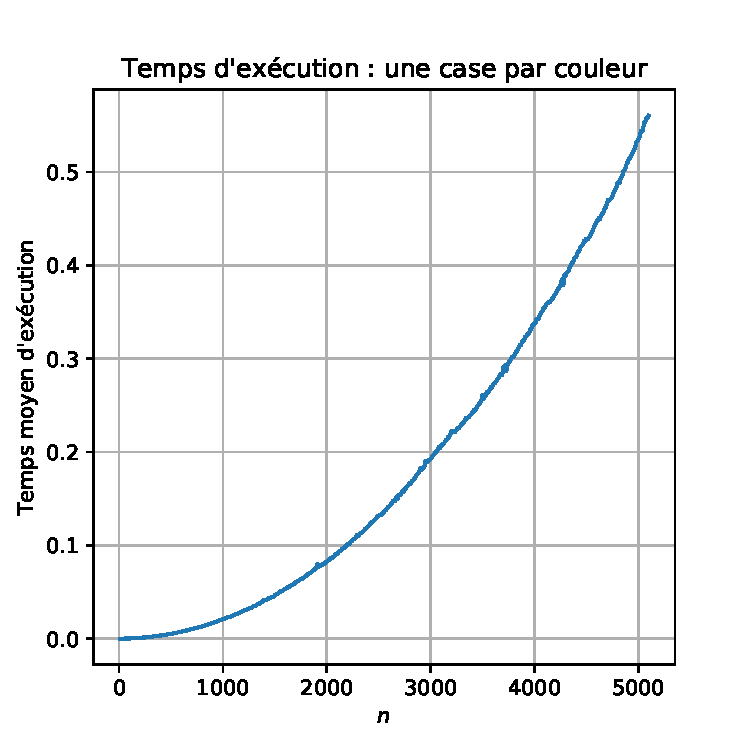
\includegraphics[width=0.5\textwidth]{TempsGraphe.pdf} & 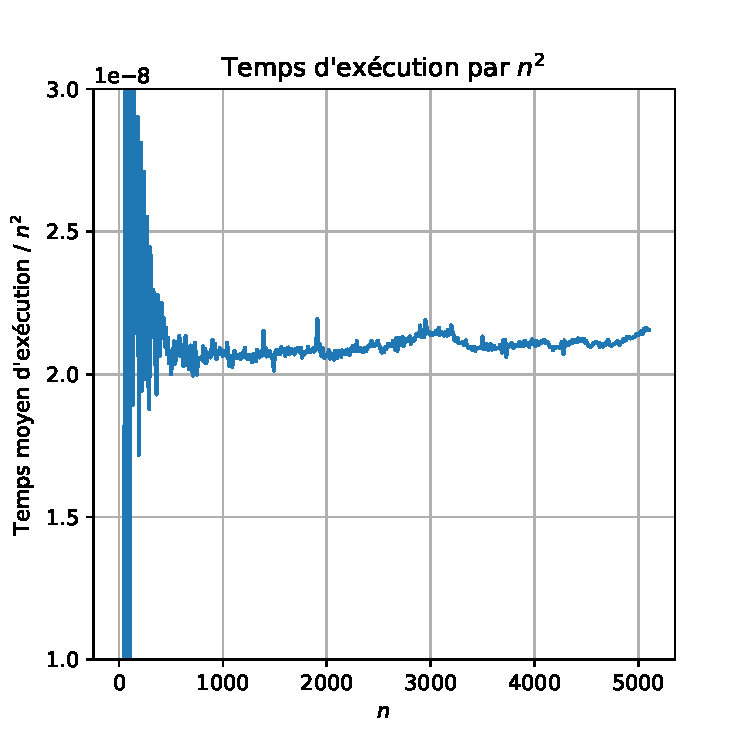
\includegraphics[width=0.5\textwidth]{TempsGrapheN2.pdf} \tabularnewline
(a) & (b) \tabularnewline
\end{tabular}
\caption{Temps d'exécution de l'algorithme.}
\label{FigTempsGraphe}
\end{figure}

Il est à noter que les résultats représentés sur la Figure \ref{FigTempsGraphe} ne sont pas directement comparables à ceux de la Figure \ref{FigGraphes}. En effet, ici, la grille est de taille $1 \times n$, contenant donc $n$ cases, chacune avec une couleur différente, alors que, pour la Figure \ref{FigGraphes}, la grille, de taille $n \times n$, contenait $n^2$ cases de uniquement $10$ couleurs.

Pour pouvoir faire ces tests, il nous a fallu implémenter des fonctions pour désallouer la mémoire utilisée par les structures de l'algorithme afin de répéter plusieurs simulations sans avoir de fuite de mémoire. En particulier, la taille de la structure qui stocke la solution devient rapidement importante lorsque $n$ croit. Comme dans les tests de la Section \ref{SecAuPlusProche}, nous avons désactivé l'écriture de la solution en disque pour éviter l'écriture de grands fichiers, couteuse en temps et en mémoire.

\subsection{Solution naïve dans le cas général}

Avant d'avoir vu l'algorithme précédent pour le cas d'un vecteur à une case par couleur, on a cherché à utiliser la structure de graphe pour coder un solveur très naïf pour le cas général de grilles de taille quelconque sans contrainte sur le nombre de couleurs. Ce solveur servait notamment à tester la création des listes de circuits et ne cherchait pas à minimiser la quantité de pas ni à avoir le même comportement que l'algorithme ``au plus proche'' de la Section \ref{SecAuPlusProche}. Il s'agit simplement de parcourir la liste de circuits en faisant les déplacements correspondants à chaque circuit et d'aller d'un circuit au suivant.

On peut noter qu'il est relativement simple de modifier cette implémentation pour coder une version de l'algorithme ``au plus proche''. En effet, il suffit de, lors de la création des circuits, chercher, pour chaque sommet, son successeur à plus petite distance. Une fois le circuit fermé, on doit chercher la case non-noire la plus proche pour commencer le circuit suivant, cette recherche pouvant être faite comme dans l'algorithme circulaire, par exemple. Cependant, cette méthode ne semble pas aussi efficace que les méthodes de la Section \ref{SecAuPlusProche}, notamment la méthode par AVL, et, par manque de temps, on ne l'a pas implémentée.

\end{document}
